\documentclass[a4paper]{article}
\usepackage{geometry}
 \geometry{
 a4paper,
 total={170mm,257mm},
 left=20mm,
 top=20mm,
 }
\usepackage[utf8]{inputenc}
\usepackage{amsmath}
\usepackage{amsfonts}
\usepackage{amssymb}
\usepackage[x11names]{xcolor}
\usepackage{hyperref}
\usepackage{graphicx}
\usepackage{subcaption}
\usepackage[many]{tcolorbox}
\usepackage{fontawesome5}

\newcommand{\highspace}{\vspace{1.2em}\noindent}

\begin{document}

    \title{CUDA Convolution 2D}
    \author{
        \begin{tabular}{@{} l l @{}}
            Alberto Ondei & 11098067 \\
            Abdullah Javed & 10764782 \\
            Andrea Valentini & 11010856
        \end{tabular}
    }
    \maketitle

    \section{Experimental setup}
    The 2D convolution algorithm was implemented in CUDA using two approaches: a naive implementation and a tiled implementation. Both implementations were tested on a Google Colab GPU (specifically, a Tesla T4).

    \highspace
    Development was done on student notebooks running Ubuntu 24.04 (native) as the operating system. The IDE used to develop the project was CLion. Since none of the team has a GPU, the testing and execution was done on the Google Colab workspace. The project was divided into several tasks to ensure that each team member could work on the project.

    \section{Performance measurements}
    The performance of the two implementations was measured for different input sizes and block sizes.

    \begin{figure}[!htp]
        \centering
        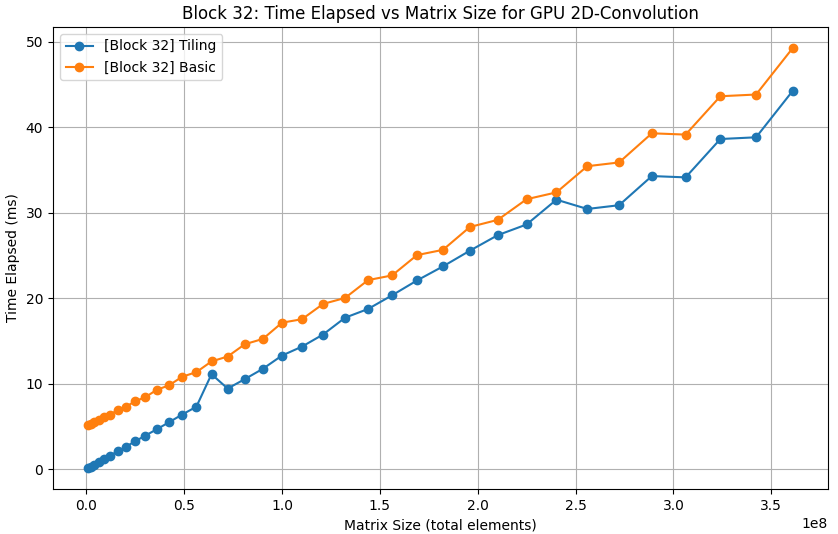
\includegraphics[width=.8\textwidth]{block32-cropped.png}
        \caption{2D convolution, with a block size of 32 (tiling or not).}
    \end{figure}

    \newpage

    \begin{figure}[!htp]
        \centering
        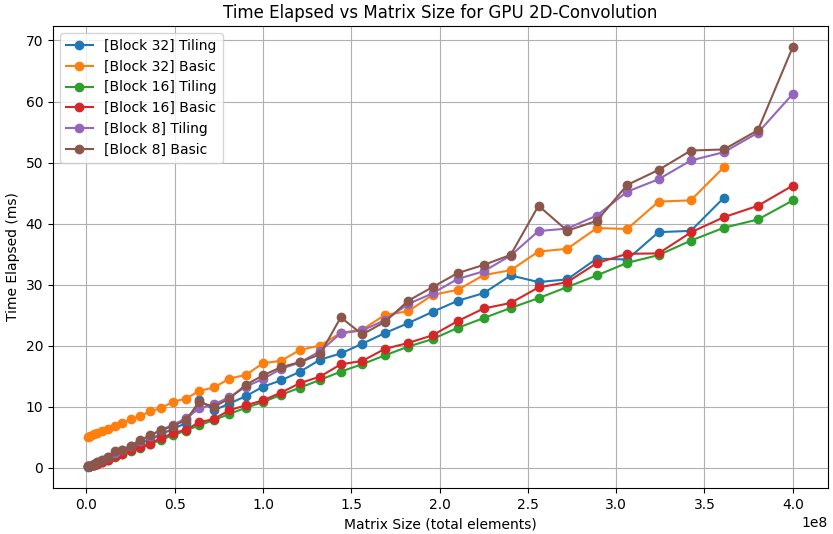
\includegraphics[width=.8\textwidth]{all-compare-cropped.png}
        \caption{2D convolution, with different block sizes (8, 16 and 32).}
    \end{figure}

    \noindent
    As the figures show, tiling execution is faster, especially for larger input matrices, due to reduced global memory accesses and efficient use of shared memory. Instead, the naive implementation shows an increase in execution time as the matrix size increases.

    \highspace
    About the block size, we can say that:
    \begin{itemize}
        \item $8 \times 8$: limited performance due to inefficient use of resources.

        \item $16 \times 16$: a balanced choice that offers good performance across matrix sizes (especially for the tiling choice, which is the faster method).
        
        \item $32 \times 32$: best for large inputs, maximizes GPU computation, but can cause contention on small problems.
    \end{itemize}
    The warm-up makes benchmarks more realistic, reducing cold start effects and improving measurement consistency.

    \section{Explanation of design choices}
    The goal is to perform the 2D convolution between a matrix and a parametric mask as efficiently as possible on the GPU.
    
    \highspace
    There are two implementations, with tiling and without tiling, in the version with tiling we assigned the same tiling size to the block and analyzed as sizes $8 \times 8$, $16 \times 16$, $32 \times 32$.
    We analyzed the same sizes in the no tiling version to see the differences using the same size blocks with and without tiling.

    \highspace
    Tiling divides the input image into small blocks (tiles) that are loaded into shared memory. Each block is processed by a group of threads, reducing the number of accesses to slower global memory. Threads within a block load data about the tile into shared memory, perform calculations on the portion of the image, and then write the results to global memory. Synchronization between threads ensures that all necessary data is loaded into shared memory before the calculations are performed.

    \highspace
    To ensure accurate performance measurements, we included a warm-up phase before benchmarking the kernel execution. This phase was critical to stabilize the system state and eliminate the cold start effect. During warmup, the necessary data and instructions were loaded into the cache, reducing cache misses and ensuring consistent results. It also allowed the CUDA runtime to allocate and initialize device memory, minimizing the impact of initialization overhead. The warm-up phase also helped the GPU and system reach a stable state, preventing transient activity from affecting the results. Overall, it allowed us to obtain accurate and reliable performance measurements that reflected the steady-state performance of our kernel.
\end{document}
